\clearpage
\appendix

\chapter{UML diagrams\label{cha:algorithm-UML-diagrams}}

\begin{figure}[htb]
    \centering
    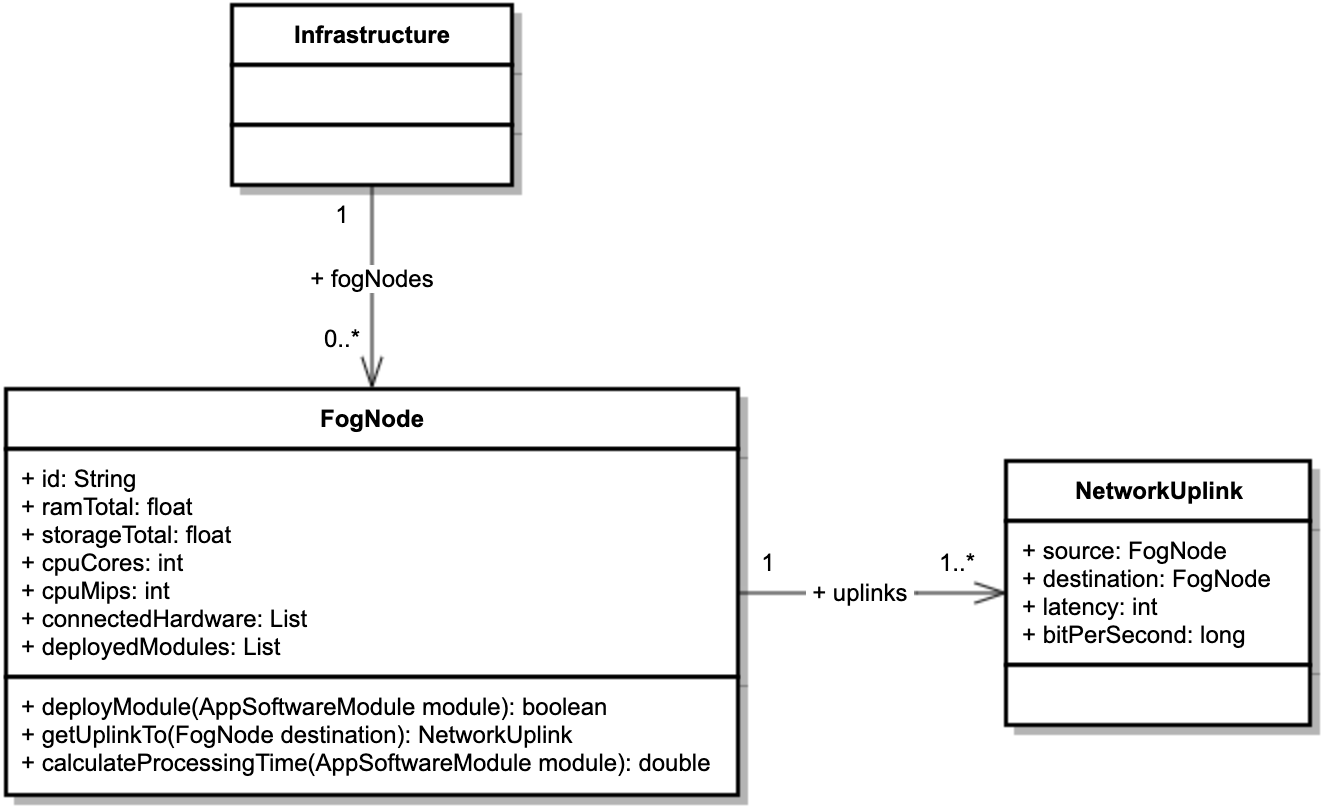
\includegraphics[width=1.0\textwidth]{algorithm-classdiagram-infrastructure}
    \caption{Class diagram representing the scheduling algorithm's infrastructure}
    \label{fig:classdiagram-infrastructure}
\end{figure}

\begin{figure}[htb]
    \centering
    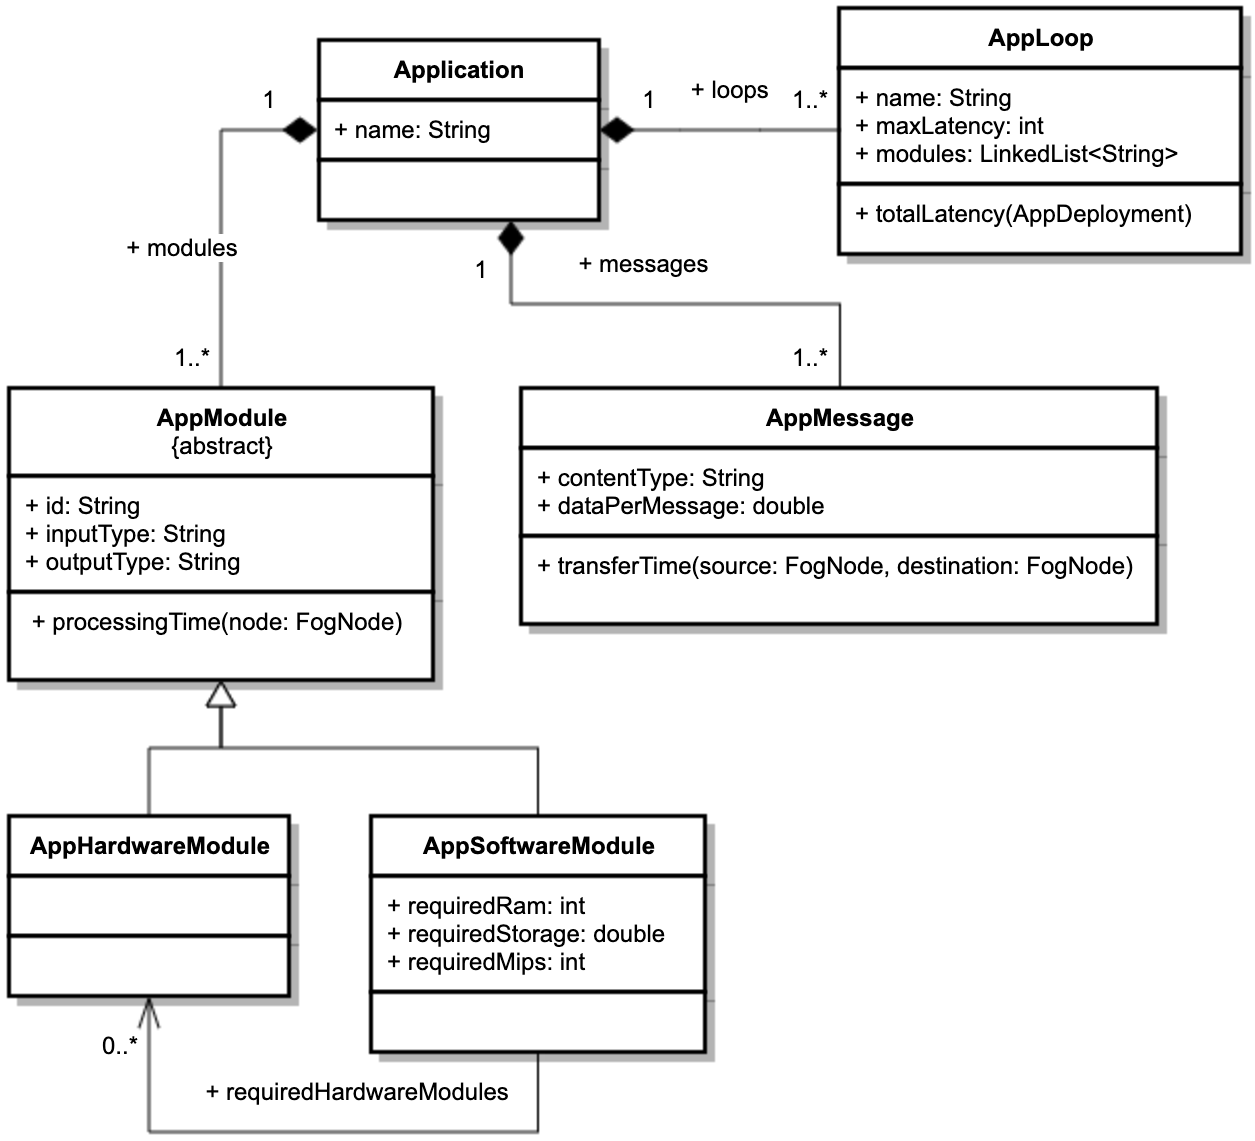
\includegraphics[width=1.0\textwidth]{algorithm-classdiagram-application}
    \caption{Class diagram representing the scheduling algorithm's application}
    \label{fig:classdiagram-application}
\end{figure}

\begin{figure}[htb]
    \centering
    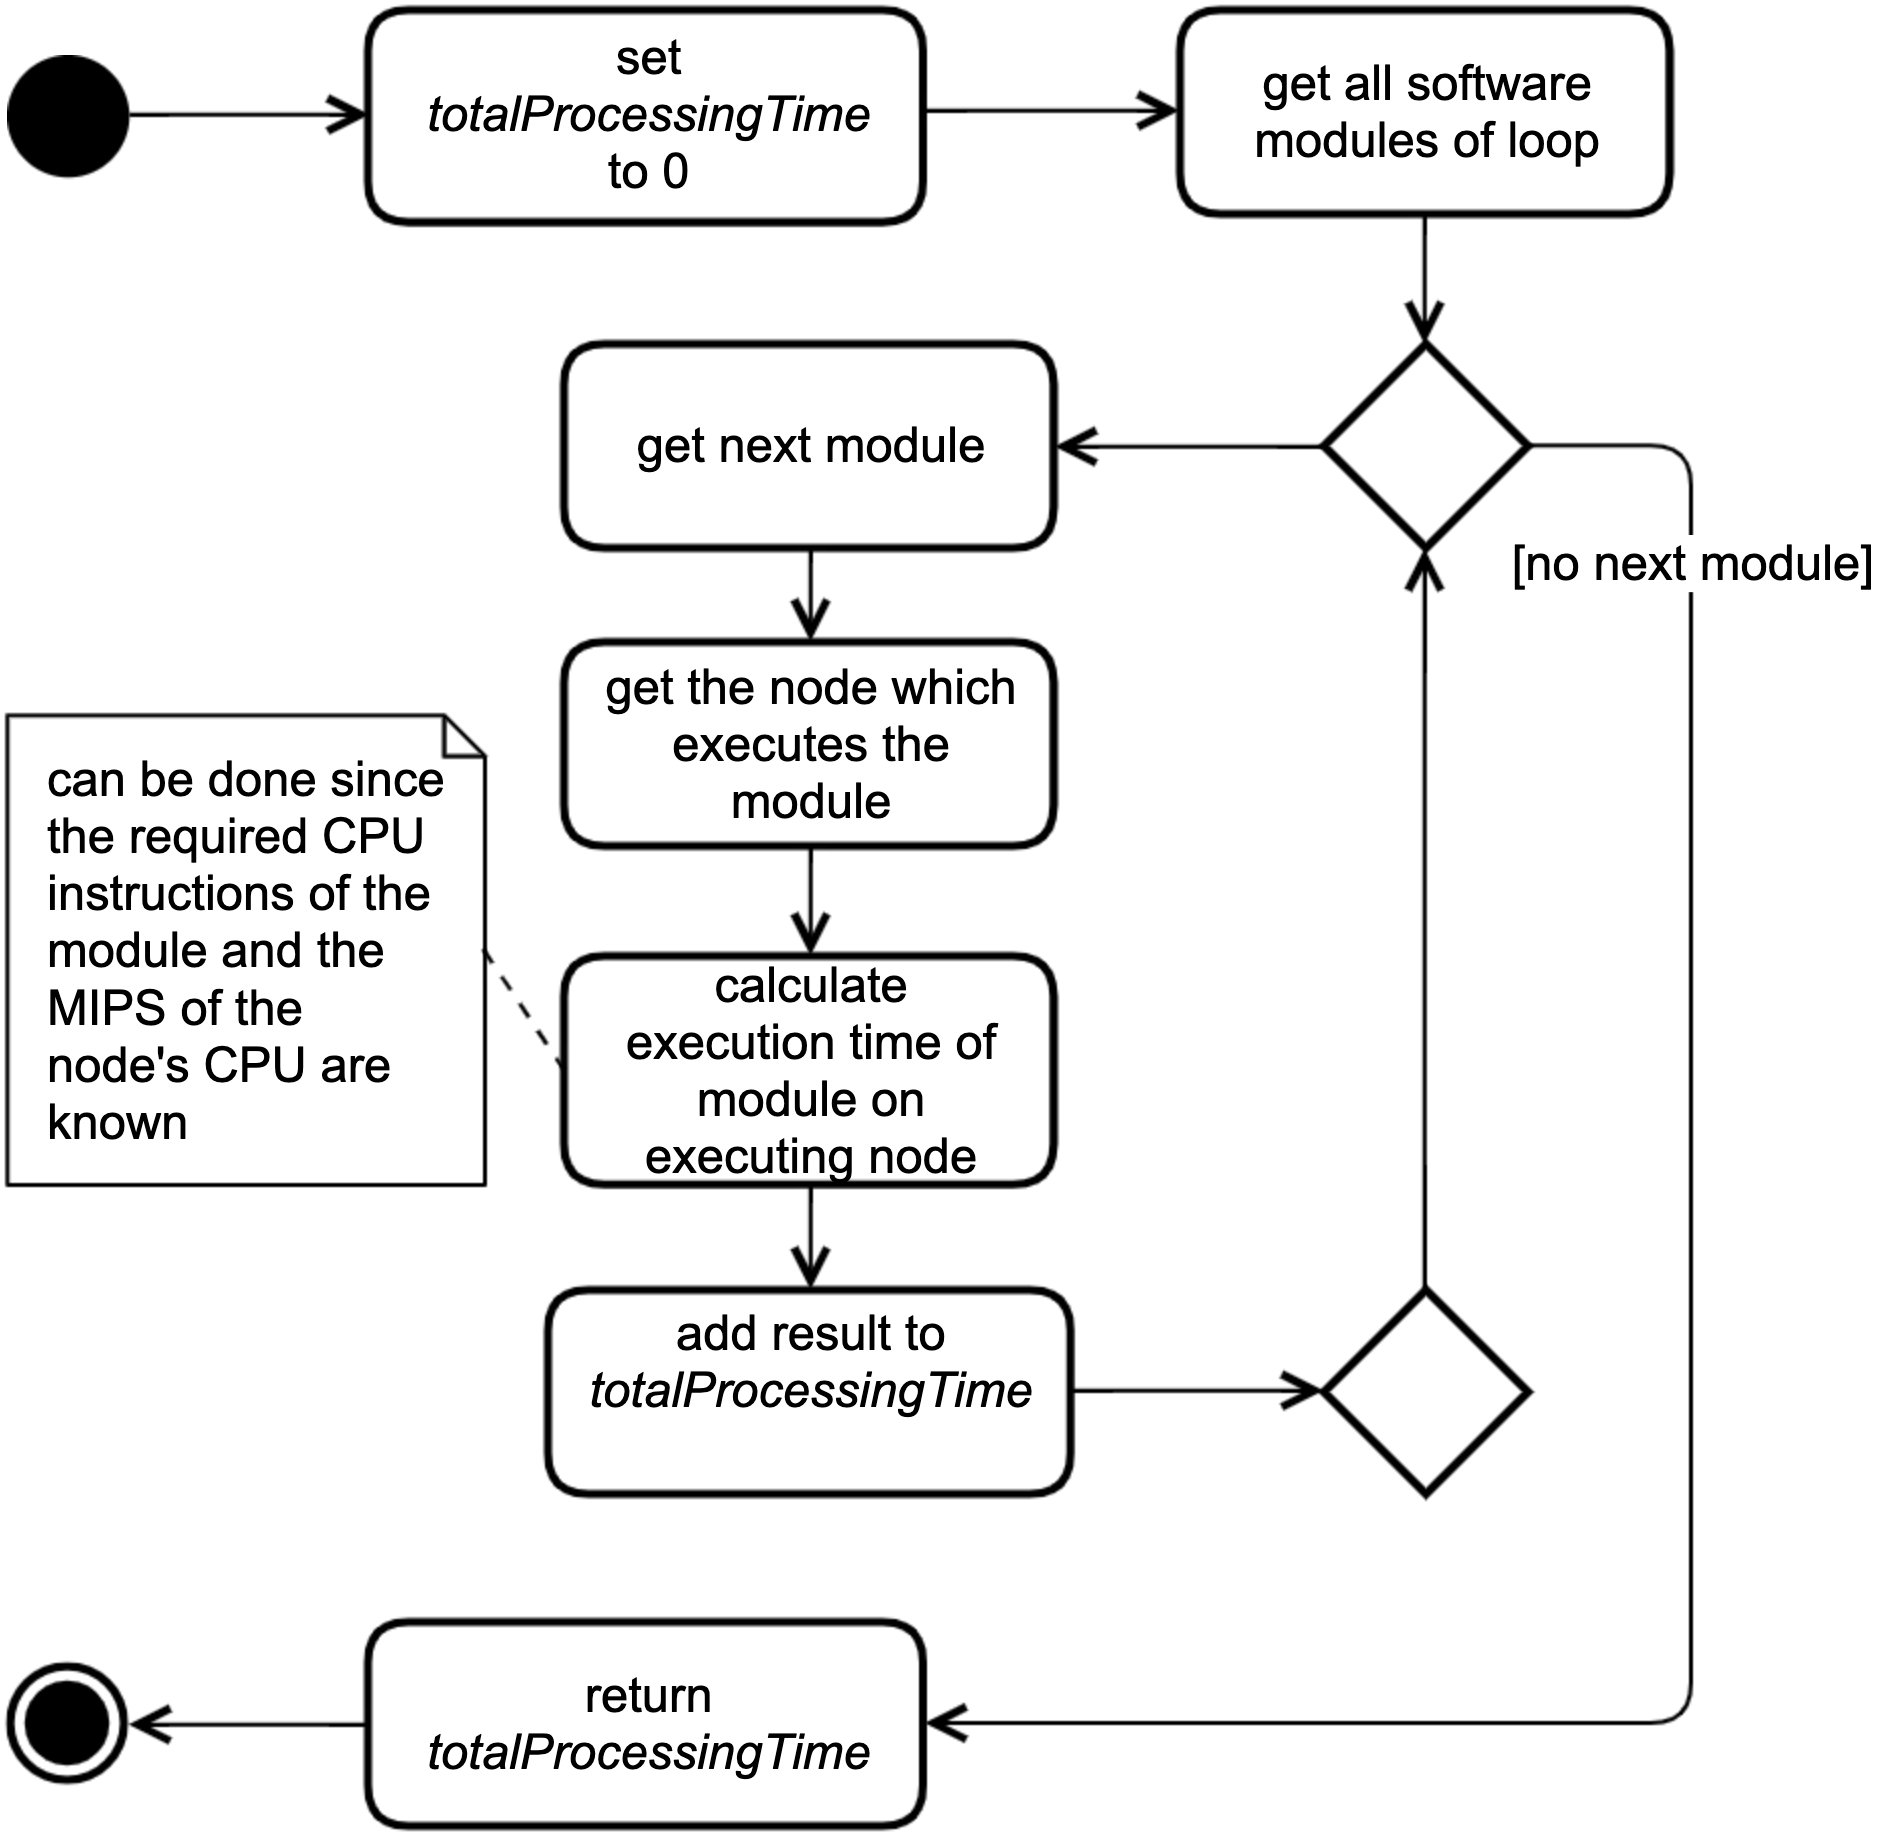
\includegraphics[width=0.9\textwidth]{algorithm-activitydiagram-latency-processing}
    \caption{Activity diagram for calculating the total task execution time of a loop}
    \label{fig:algorithm-activitydiagram-latency-processing}
\end{figure}

\begin{figure}[htb]
    \centering
    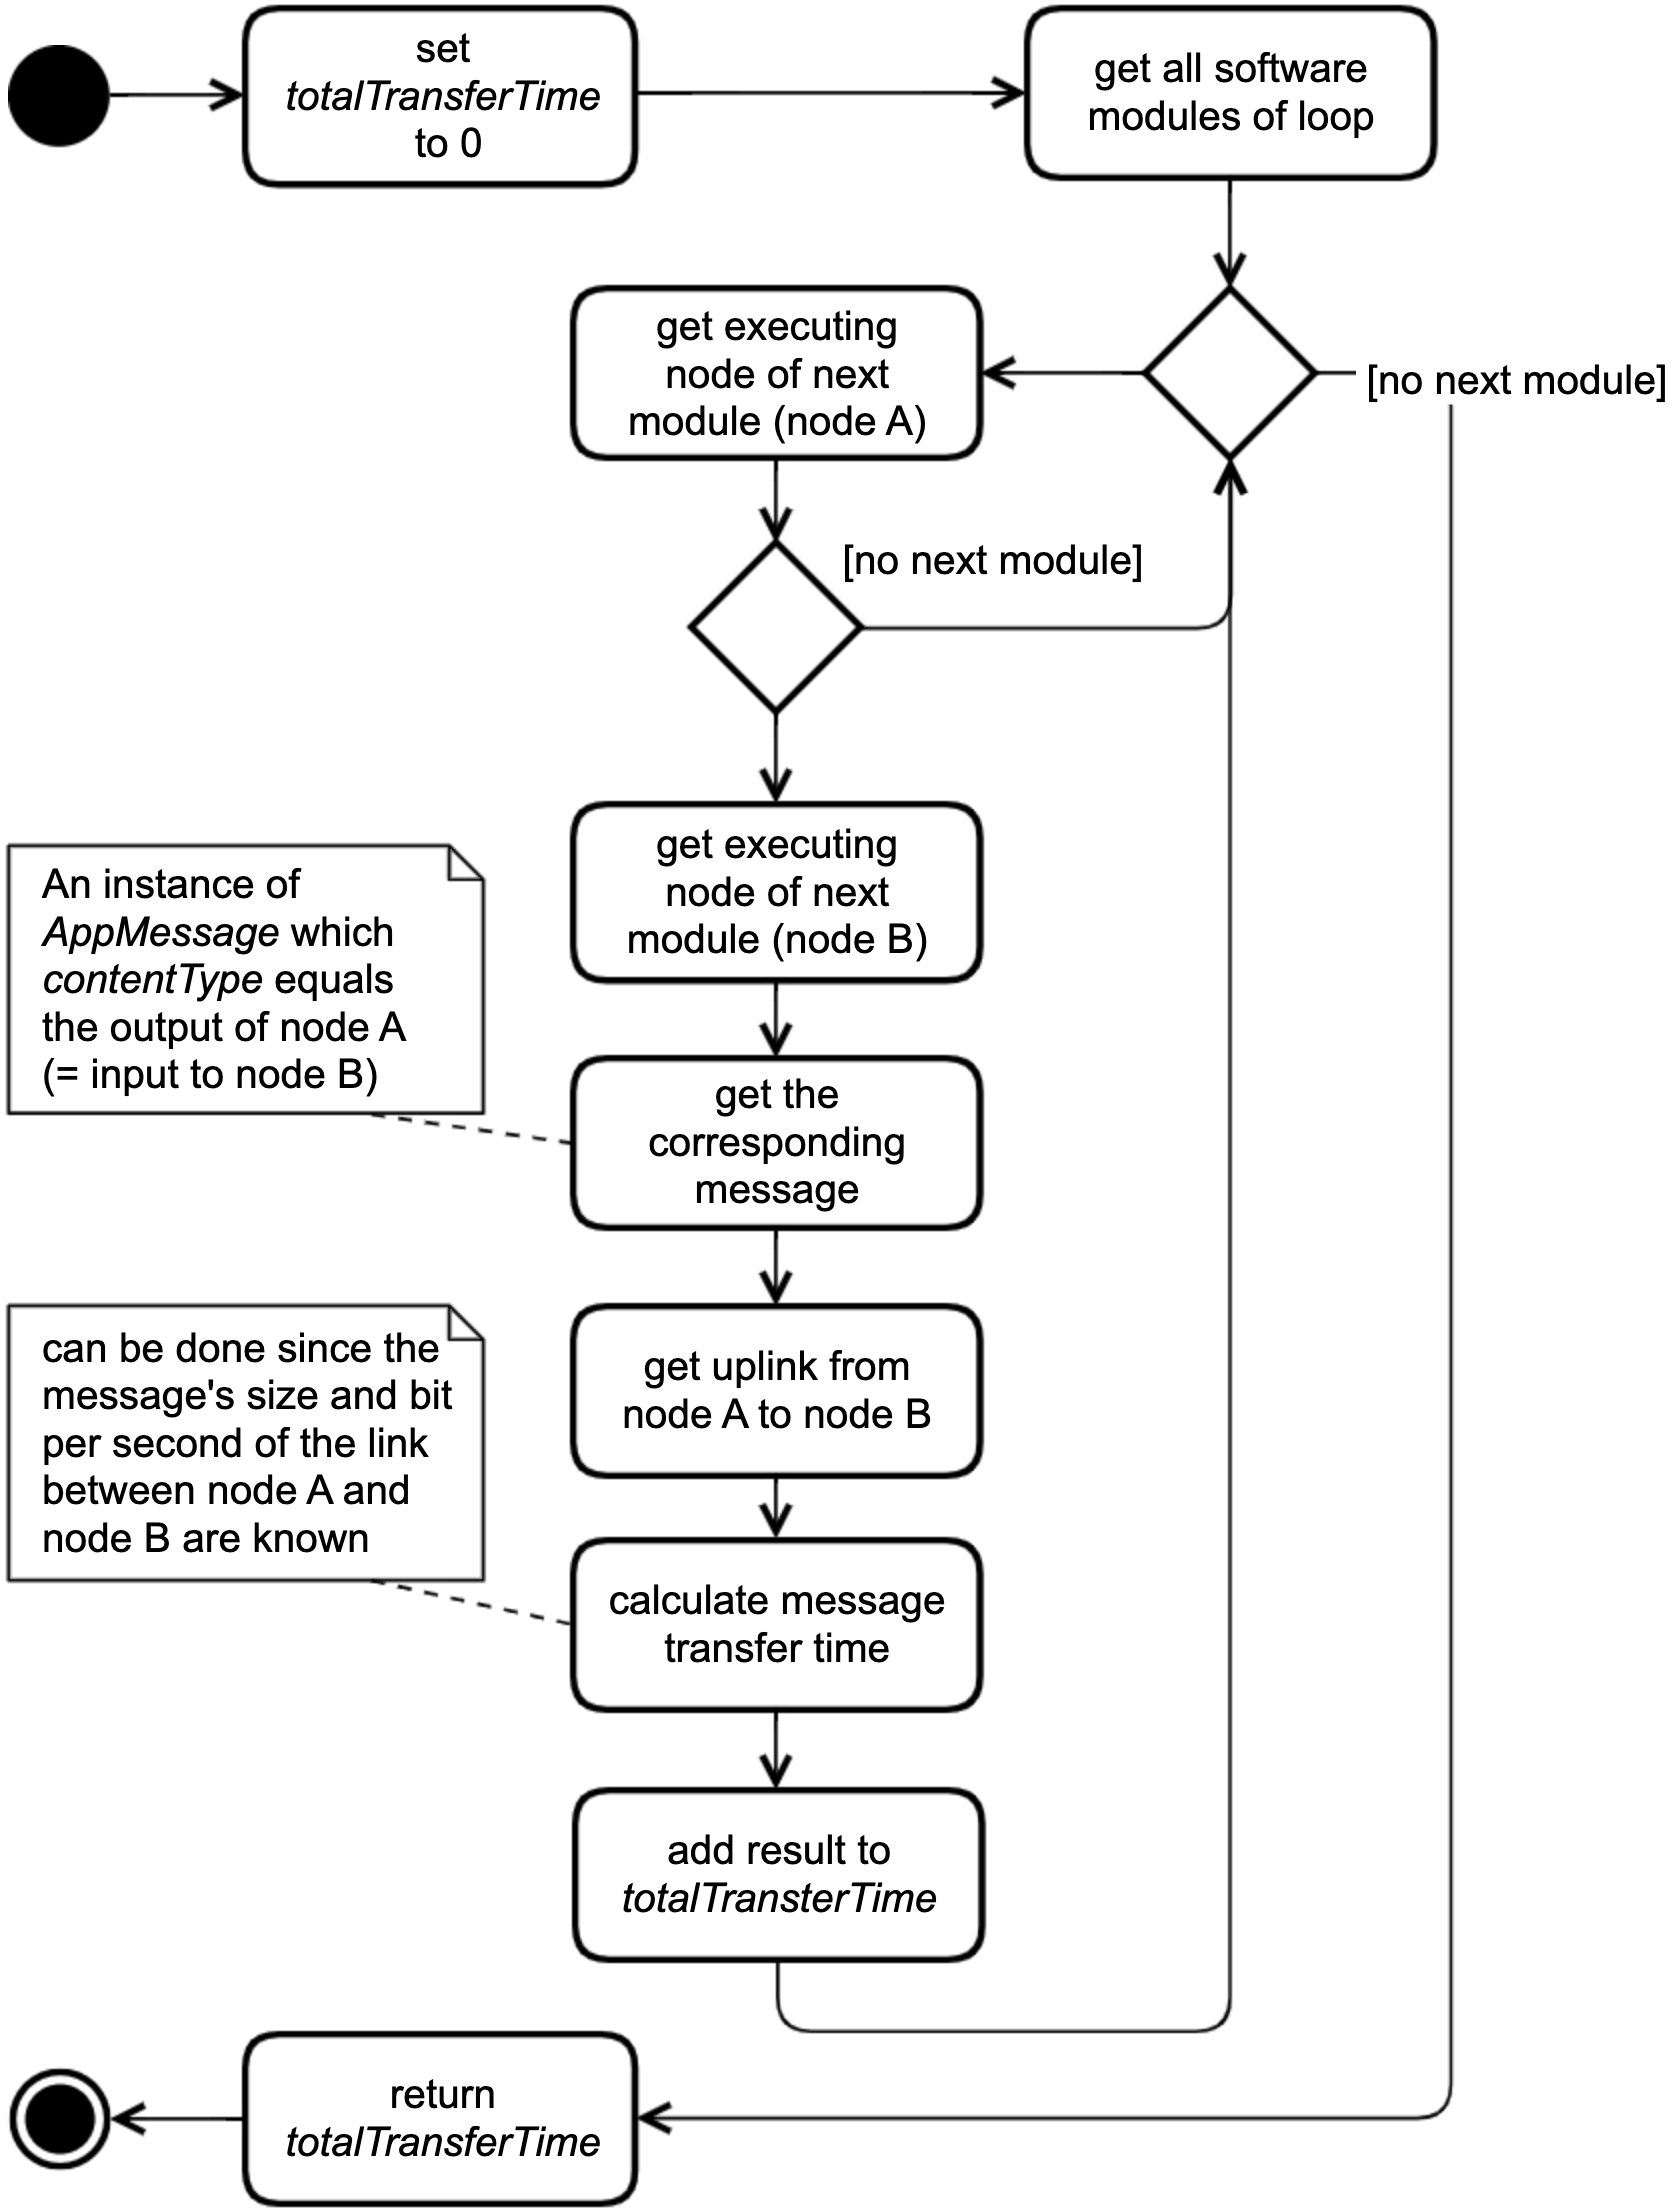
\includegraphics[width=0.9\textwidth]{algorithm-activitydiagram-latency-transfer}
    \caption{Activity diagram for calculating the total transfer time of messages between nodes of a loop}
    \label{fig:algorithm-activitydiagram-latency-transfer}
\end{figure}



\begin{figure}[htb]
    \centering
    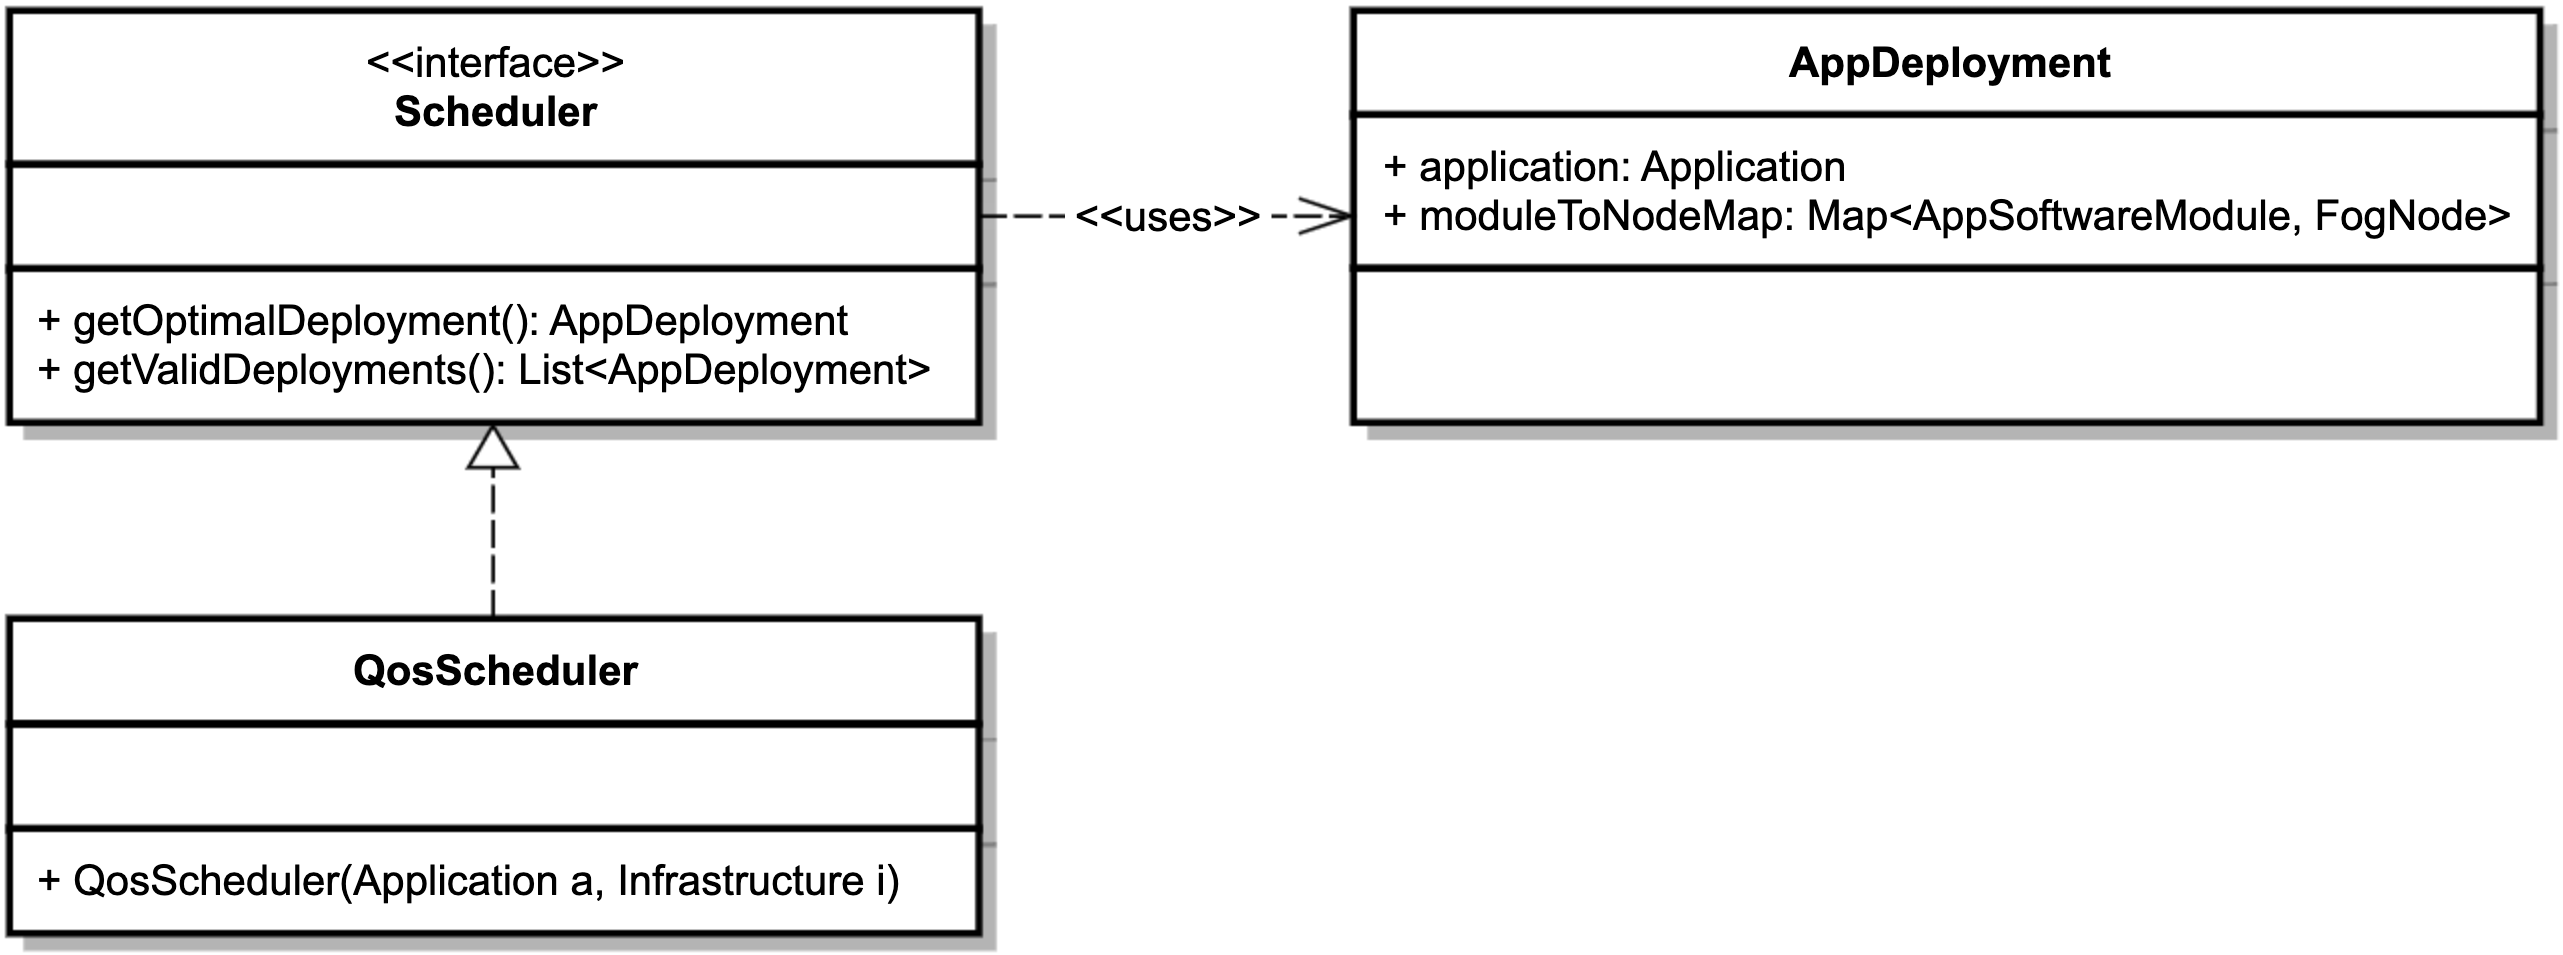
\includegraphics[width=1.0\textwidth]{algorithm-classdiagram-scheduler}
    \caption{Class diagram representing the QoS scheduler}
    \label{fig:classdiagram-qosscheduler}
\end{figure}

\begin{figure}[htb]
    \centering
    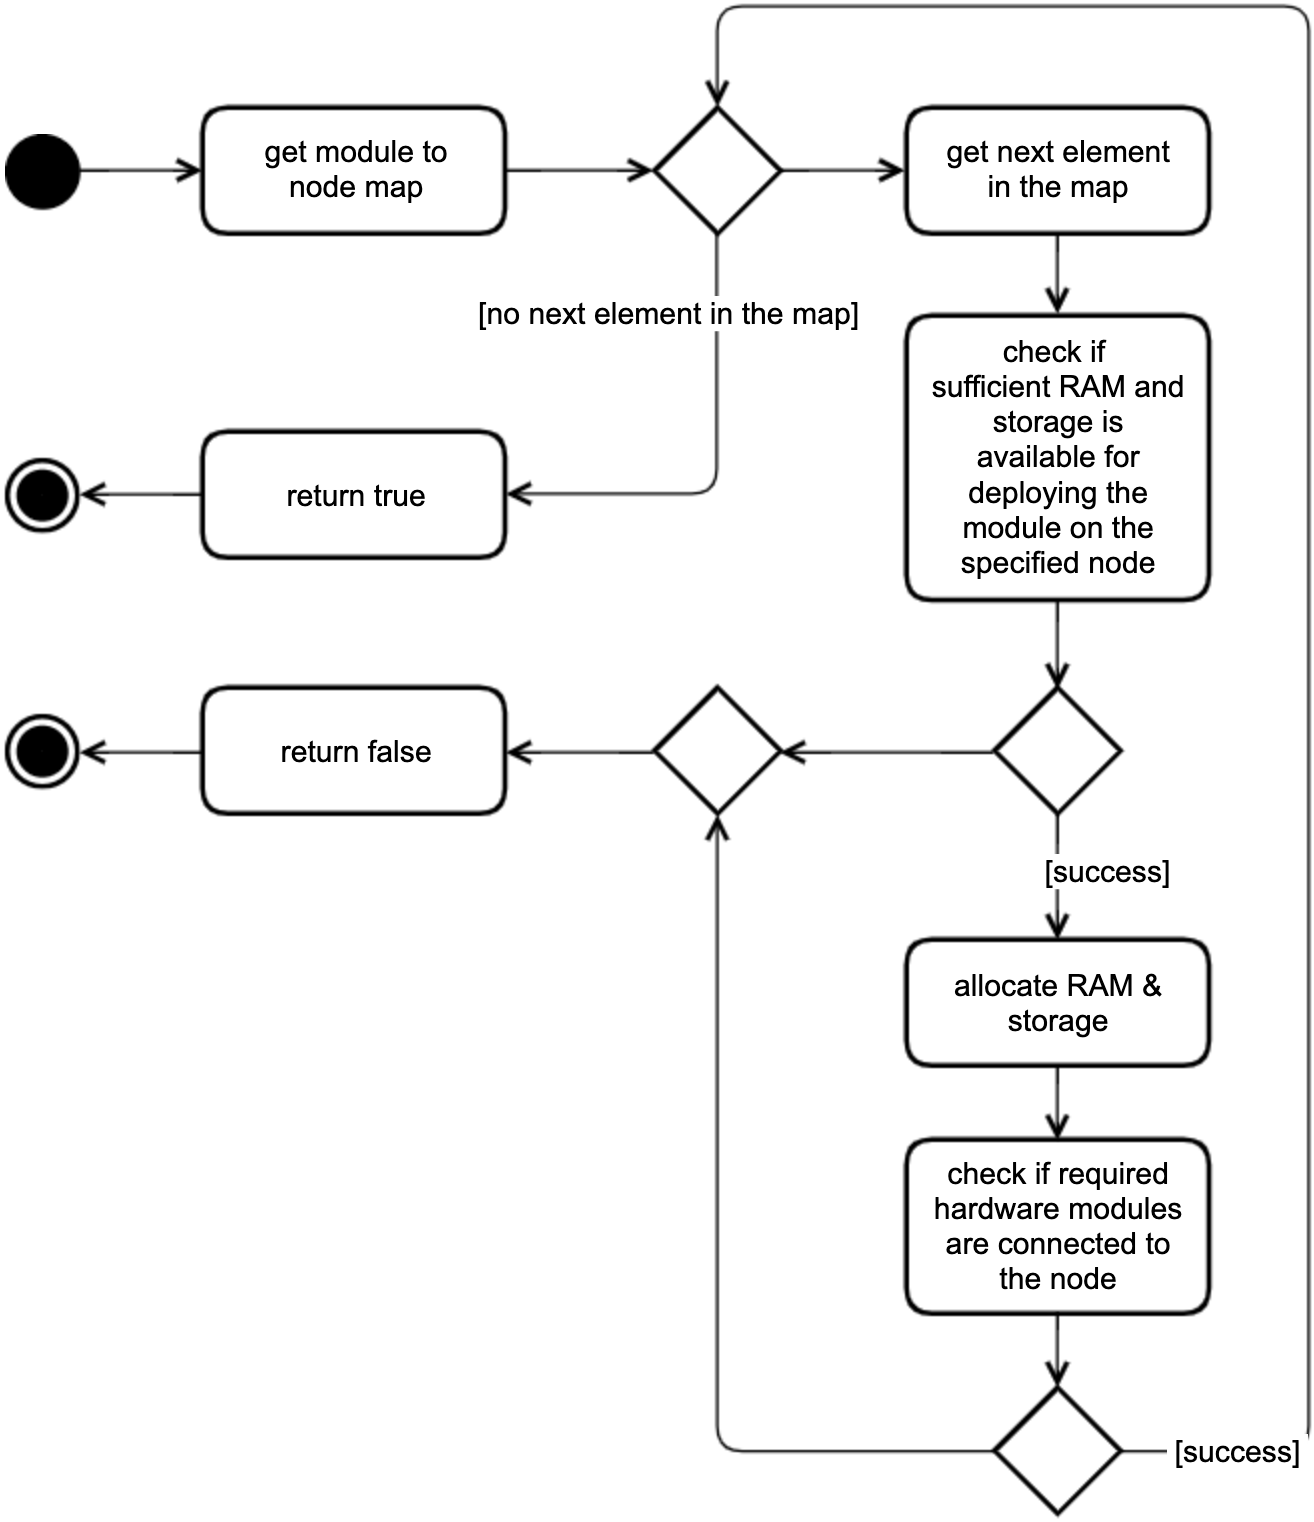
\includegraphics[width=0.9\textwidth]{algorithm-activitydiagram-hardware}
    \caption{Activity diagram for validating hardware requirements}
    \label{fig:algorithm-activitydiagram-hardware}
\end{figure}


\begin{figure}[htb]
    \centering
    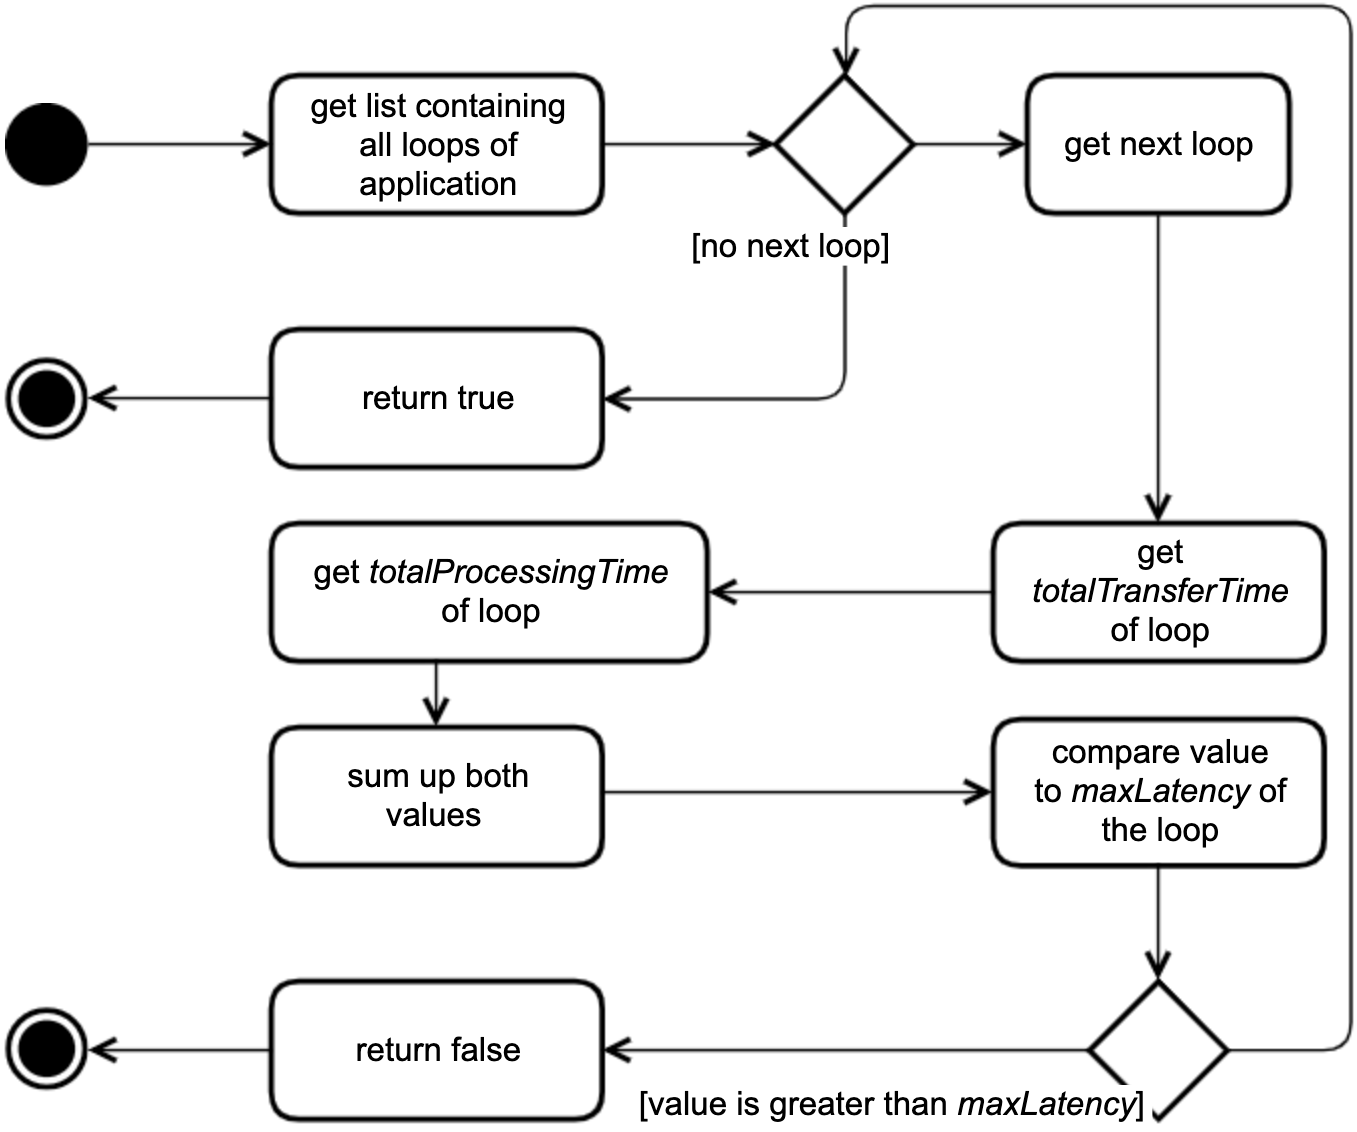
\includegraphics[width=0.9\textwidth]{algorithm-activitydiagram-latency}
    \caption{Activity diagram for validating latency requirements}
    \label{fig:algorithm-activitydiagram-latency}
\end{figure}

\begin{figure}[htb]
    \centering
    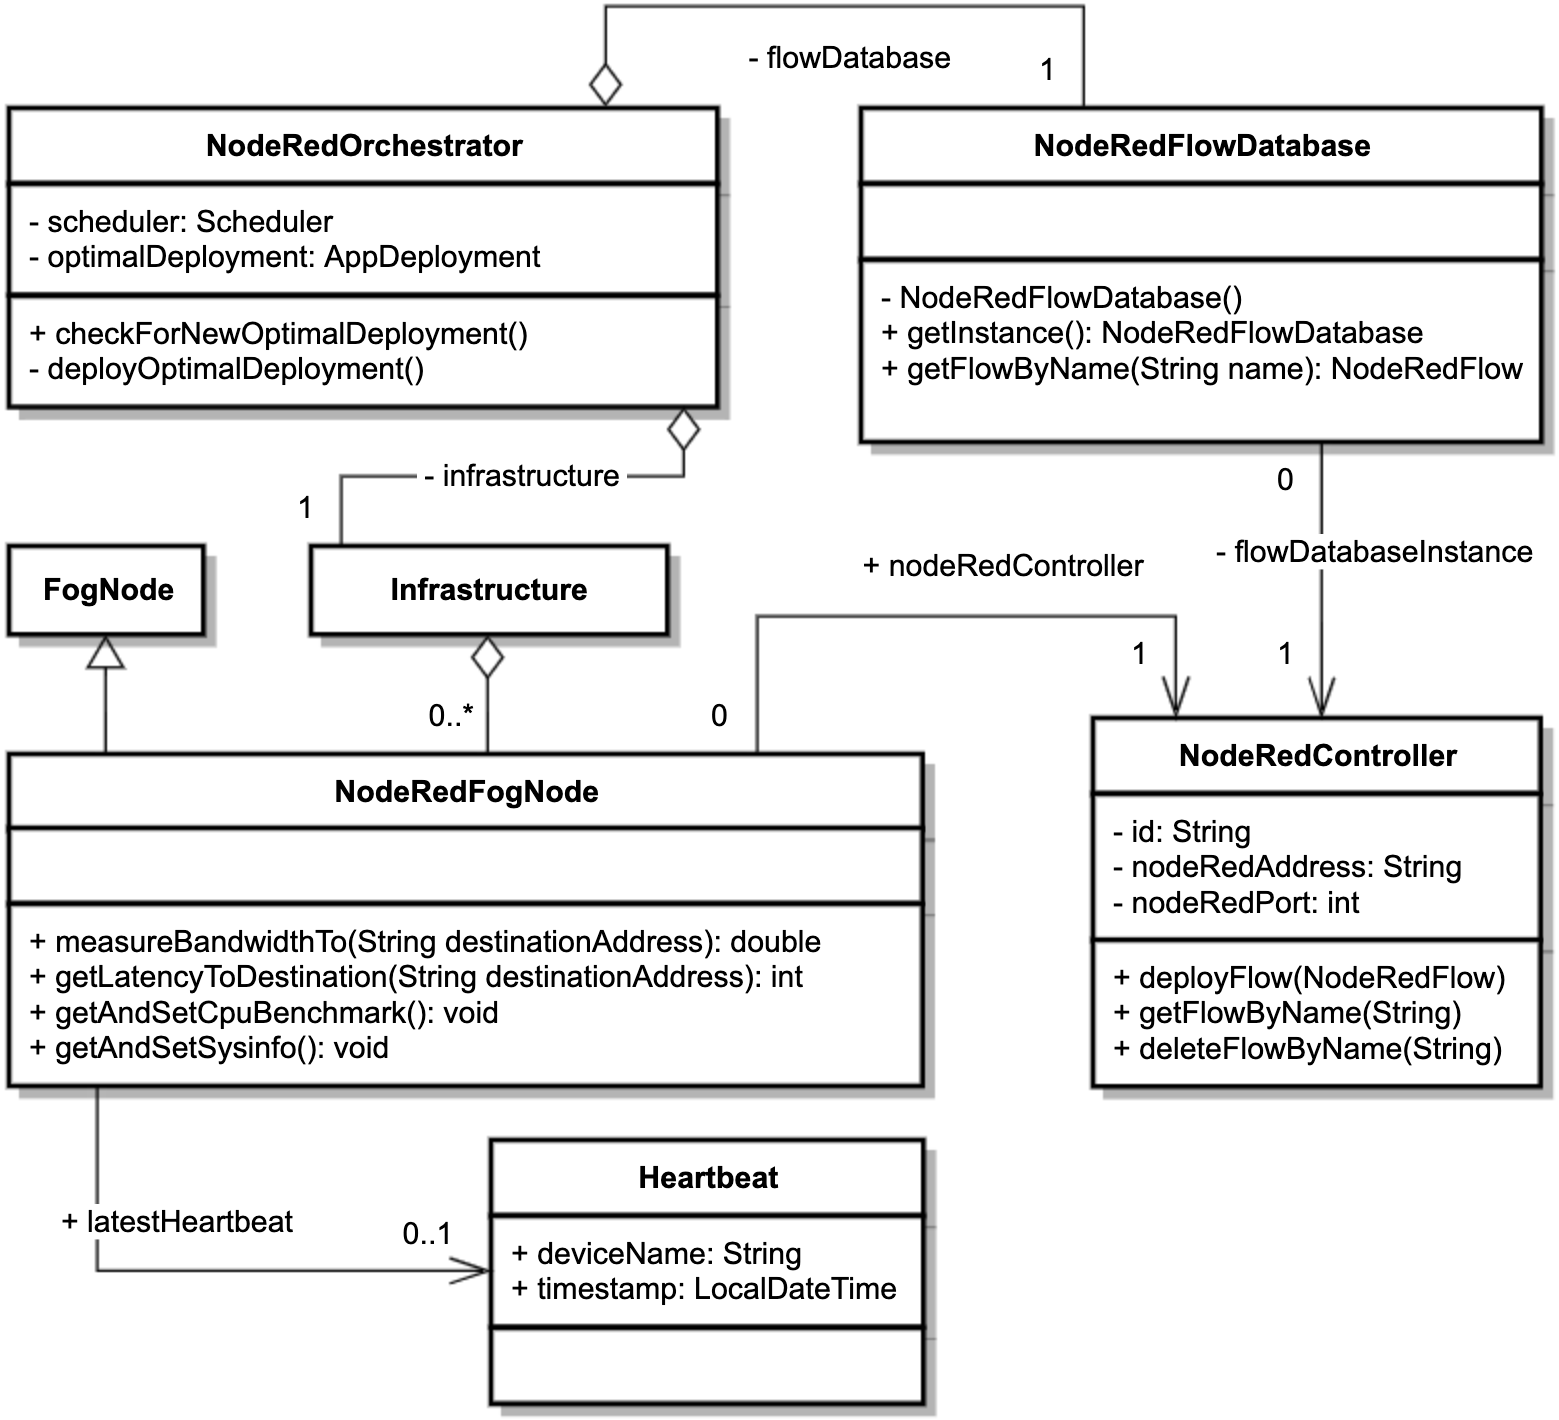
\includegraphics[width=1.0\textwidth]{orchestrator-classdisgram}
    \caption{Class diagram of the Orchestrator}
    \label{fig:orchestrator-classdisgram}
\end{figure}

\clearpage
\chapter{Screenshots\label{cha:appendix-screenshots}}
\begin{figure}[htb]
    \centering
    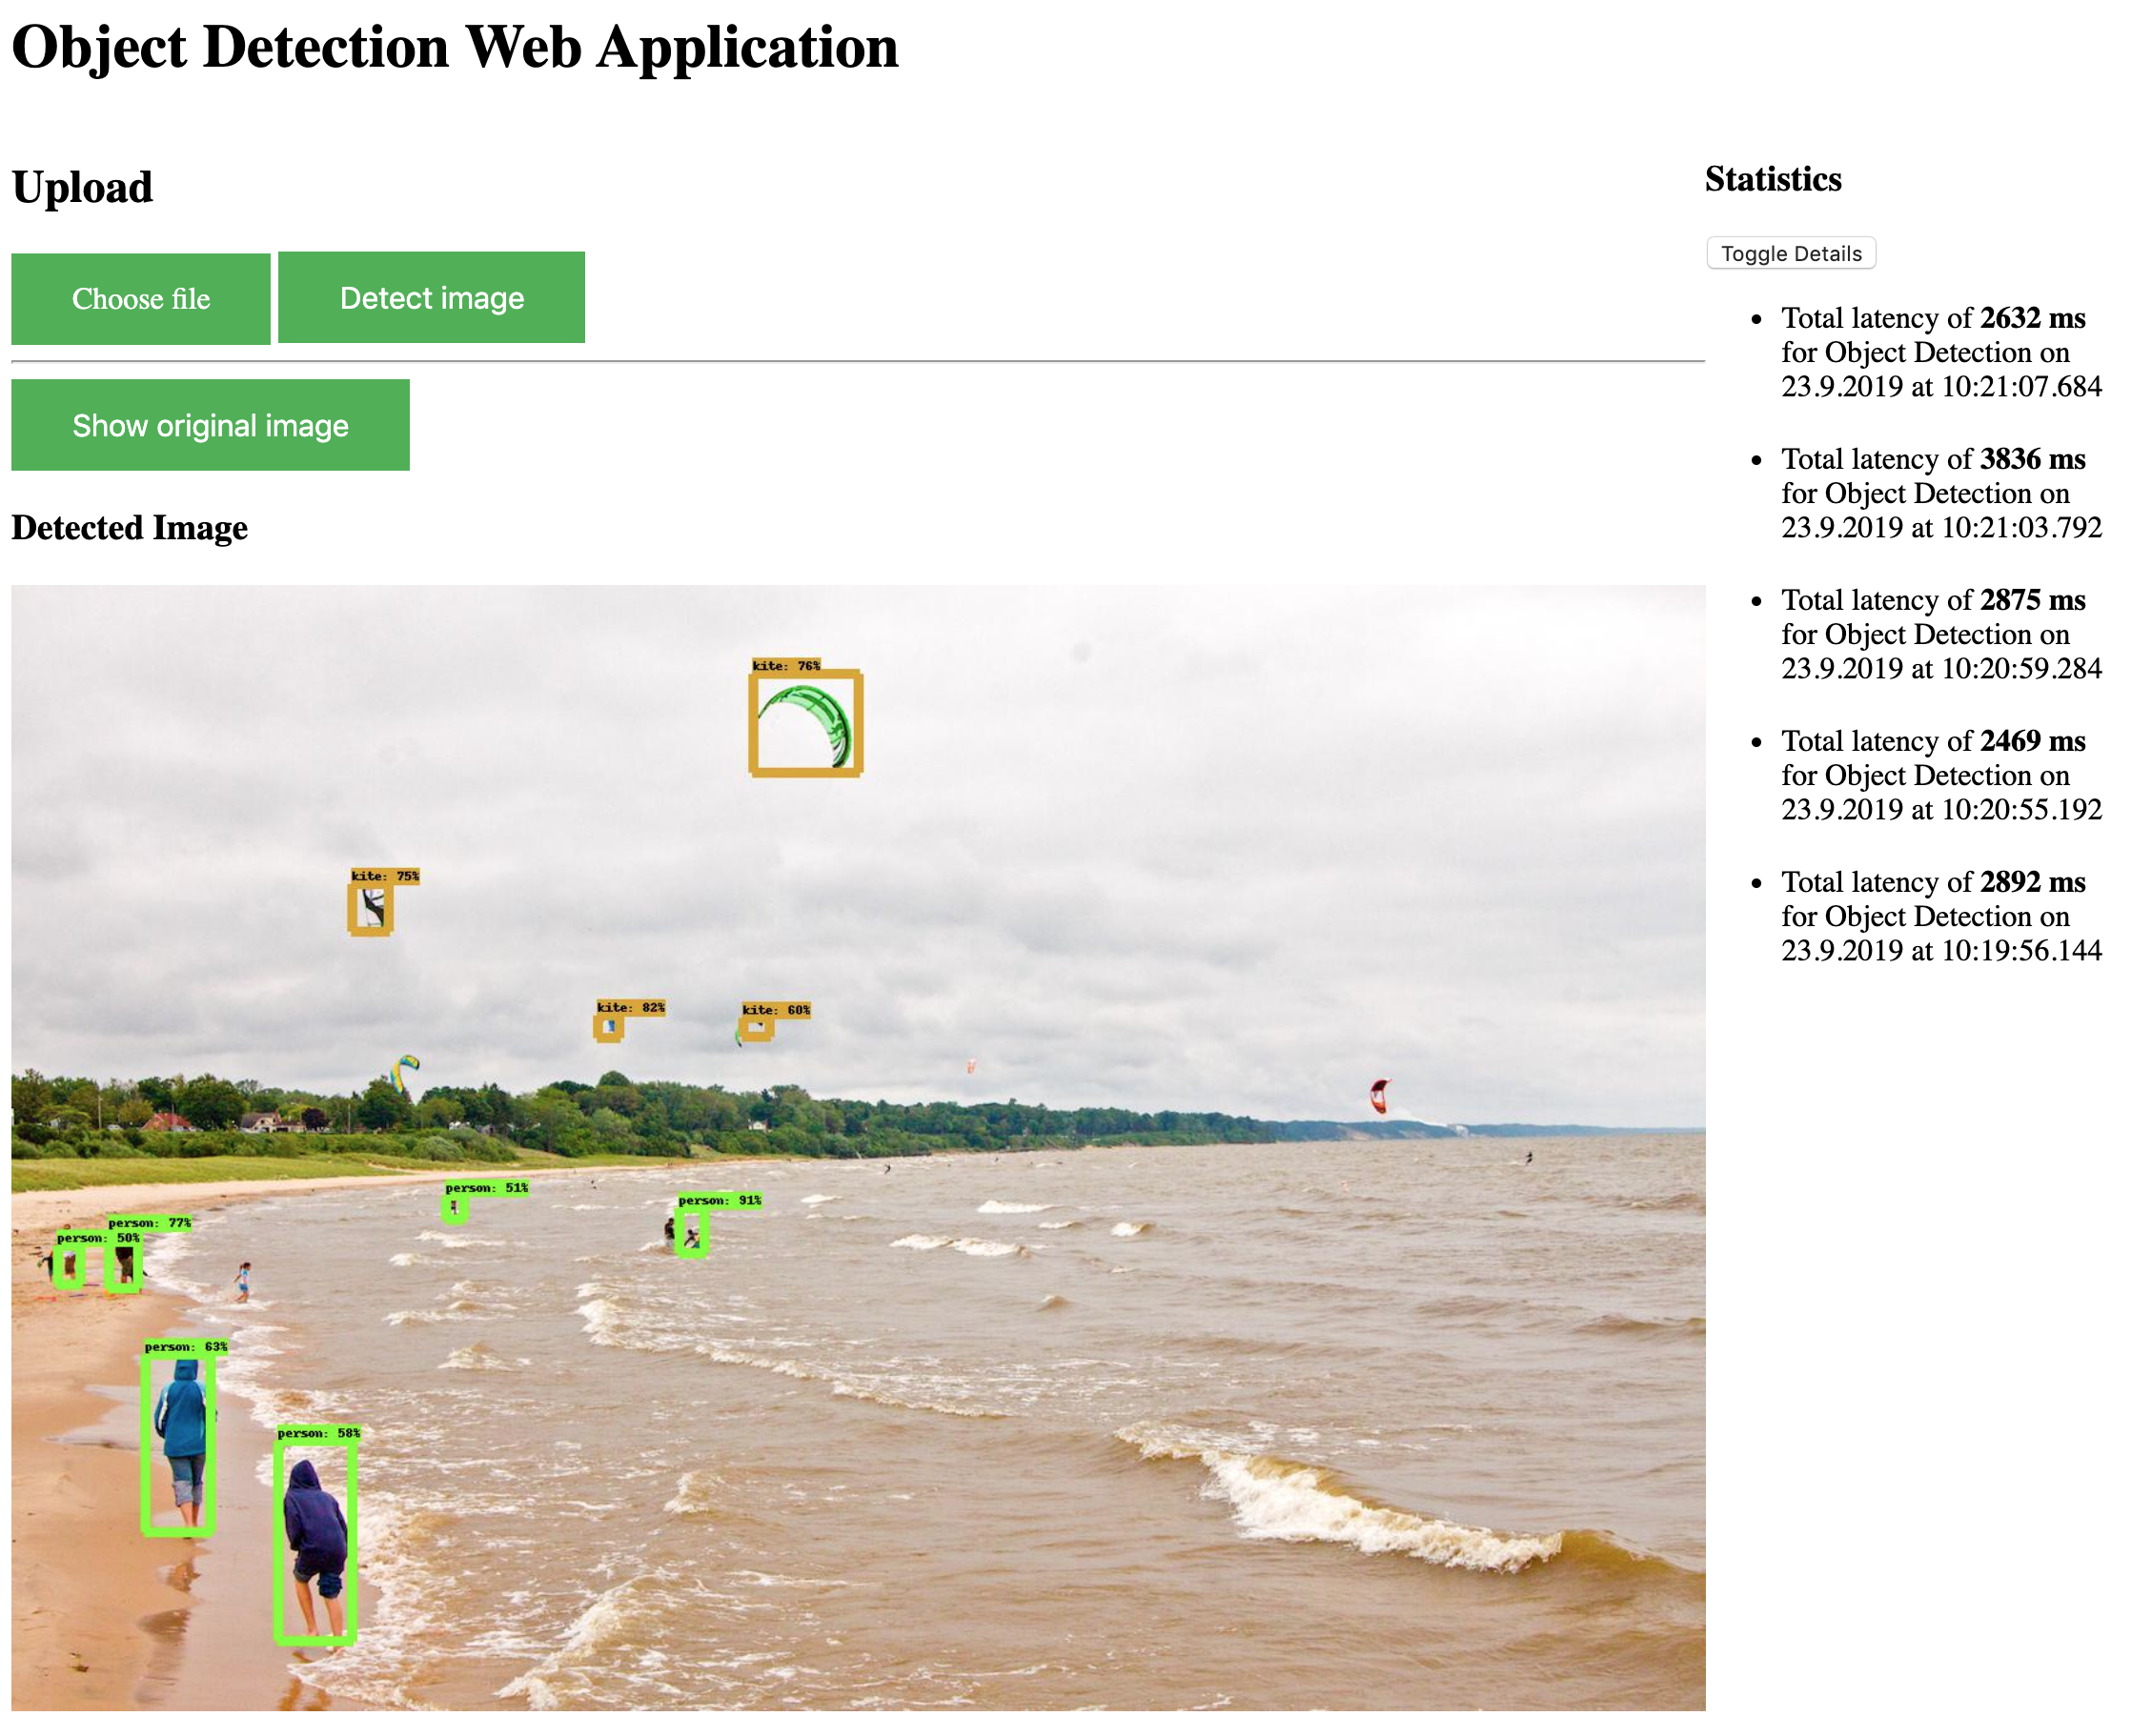
\includegraphics[width=1.0\textwidth]{object-detection-webapp-screenshot}
    \caption{Screenshot of the Object Detection Web Application}
    \label{fig:object-detection-webapp-screenshot}
\end{figure}